% Compile with
%   lualatex Ratchet.tex
% (no minted, so no --shell-escape needed)
%
% Second talk on how we work: exclusively the ratchet project
% (~/Code/research/ratchet, August 2026), from which the runs originated.

\documentclass[11pt,aspectratio=169]{beamer}
\setbeamertemplate{navigation symbols}{}
\usepackage{background}
\usepackage{booktabs}
\usepackage{tikz}
\usetikzlibrary{arrows.meta, positioning, fit, backgrounds, calc}
\usepackage{fontspec}
\setmonofont[Scale=0.85]{DejaVu Sans Mono}
\usepackage[english]{babel}
\usepackage{csquotes}
\usepackage{amsmath, amssymb}
\usepackage{xcolor}
\usepackage{hyperref}
\hypersetup{colorlinks=true, linkcolor=blue, urlcolor=blue}

\definecolor{darkgreen}{rgb}{0.0,0.4,0.0}
\definecolor{darkblue}{rgb}{0.1,0.1,0.5}
\definecolor{darkred}{rgb}{0.5,0.0,0.0}
\definecolor{gray}{rgb}{0.35,0.35,0.35}
\definecolor{nutzer}{rgb}{0.75,0.2,0.1}
\definecolor{sitzung}{rgb}{0.1,0.35,0.7}
\definecolor{lauf}{rgb}{0.0,0.5,0.3}
\setbeamercolor{title}{fg=white}
\setbeamercolor{author}{fg=white}
\setbeamercolor{date}{fg=white}
\setbeamertemplate{blocks}[rounded][shadow=true]

\newcommand{\datei}[1]{\texttt{#1}}
\tikzset{
  box/.style={draw, rounded corners, thick, align=center, inner sep=5pt, font=\small},
  pfeil/.style={-{Stealth[length=2.5mm]}, thick},
}

\title{How it started}
\subtitle{The ratchet project: an autonomous research run on Muller's ratchet}
\author{Peter Pfaffelhuber}
\date{Freiburg, September 2026}

\begin{document}

\backgroundsetup{scale=1, color=black, opacity=1, angle=0, contents={\vspace*{3cm}\hspace*{-10cm}
\includegraphics[width=1.80\paperwidth,height=1.33\paperheight]{hintergrund_vortrag1.pdf}}}
\setbeamertemplate{background}{\BgMaterial}
\begin{frame}
  \titlepage
\end{frame}

\setbeamertemplate{background}{}
\setbeamertemplate{footline}{%
  \hbox{\hskip 0.5cm
\includegraphics[height=0.55cm]{ufr.png}\hfill
    \usebeamerfont{footline}\color{gray}\insertframenumber\hskip 0.5cm}%
  \vskip 4pt%
}

% ------------------------------------------------------------------
\begin{frame}{The problem: the click rate of Muller's ratchet}
  \small
  An infinite system of SDEs with Fleming--Viot noise, $k=0,1,2,\dots$, $\sum_k X_k=1$:
  \[
    dX_k = \Big(\alpha\Big(\sum_j (j-k)X_j\Big)X_k + \lambda(X_{k-1}-X_k)\Big)dt
      + \sum_{\ell\neq k}\sqrt{\tfrac1\nu X_kX_\ell}\,dW_{k\ell}.
  \]
  $X_k$ is the fraction of individuals carrying $k$ deleterious mutations.
  $K^\ast(t)=\inf\{k: X_k(t)>0\}$ occasionally jumps by one: a \textbf{click}.
  \begin{itemize}
  \item Wanted: the rate $\mathfrak r=\lim_t K^\ast(t)/t$. Since
    $\mathfrak r(\alpha,\lambda,\nu)=\alpha\,\mathfrak r(1,\theta,\nu\alpha)$, there are two
    parameters: $\theta=\lambda/\alpha$ and $n=\nu\alpha$.
  \item For $n\to\infty$ this is \textbf{small noise}. The fixed point is
    $\pi=\mathrm{Poi}(\theta)$, and a click is a rare exit. Conjecture:
    $\tfrac1n\log\mathfrak r\to-V_\ast(\theta)$, with $V_\ast$ the quasi-potential.
  \item The literature closes the system into one equation for $X_0$:
    $V_{1d}(\theta)=2\theta\big[(1+\theta)\log(1+1/\theta)-1\big]$.
    The error is up to a factor of~2.
  \end{itemize}
  \begin{block}{The task}
    Get beyond the 1d heuristic. Another 1d closure is \textbf{not} progress.
  \end{block}
\end{frame}

% ------------------------------------------------------------------
\begin{frame}{What was available}
  \footnotesize
  \begin{columns}[T]
    \begin{column}{0.5\textwidth}
      \textbf{In the repository}
      \begin{itemize}
      \item our own manuscript arXiv:2606.15842 (Heinzel, P., Wakolbinger),
        PDF and \TeX
      \item \datei{ldp.tex}, \enquote{state of the discussion}: the Hamiltonian, the
        Neher--Shraiman heuristic, two checklists
      \item 93 ground-truth files: $N=10^4$, 1000 paths each up to the first click
      \item the Wright--Fisher simulation from the paper, CPU port and GPU
      \end{itemize}
      \textbf{Local, not in the repository} (\datei{\textasciitilde/bwSyncShare/Papers})
      \begin{itemize}
      \item Feng \& Kurtz, \emph{Large Deviations for Stochastic Processes}, 414 pp.
      \item Feng \& Xiong (2002): quasi-potential for Fleming--Viot, \enquote{the blueprint}
      \end{itemize}
    \end{column}
    \begin{column}{0.5\textwidth}
      \textbf{Ratchet literature} (\datei{Papers/ratchet/})
      \begin{itemize}
      \item Neher \& Shraiman (2012): the 1d heuristic
      \item Audiffren \& Pardoux (2013); Mariani, Pardoux \& Velleret (2025)
      \item Etheridge, P., Wakolbinger (2008)
      \item Dawson \& Feng (1998): LDP for Fleming--Viot \emph{with selection}
      \item Champagnat \& Hass (2023) and seven more
      \end{itemize}
      \textbf{Obtained on 13 Aug} for B4
      \begin{itemize}
      \item Conforti--Kraaij--Tonon (2), Puhalskii (2),
        Budhiraja--Dupuis--Maroulas
      \item six paywalled titles recorded as \enquote{not obtainable, do not search}
      \end{itemize}
    \end{column}
  \end{columns}
\end{frame}

% ------------------------------------------------------------------
\begin{frame}{The idea of the runs (1--3 Aug 2026)}
  \begin{itemize}
  \item \textbf{I am on vacation.} A computer in the office works alone for one week,
    running \texttt{claude -p} every four hours.
  \item \textbf{No run has a memory.} The state lives only in \datei{RESEARCH\_LOG.md}
    and in the commits. Every run reads the whole log and appends an entry.
  \item \textbf{The name says it all.} A ratchet turns in one direction only: nothing
    verified is ever given up.
  \end{itemize}
  \medskip
  \begin{columns}[T]
    \begin{column}{0.47\textwidth}
      \begin{block}{A log entry}
        \footnotesize
        \textbf{Read}: the current state\\
        \textbf{Tried}: the approach\\
        \textbf{Result}: PROVED / CONJECTURE / DEAD END\\
        \textbf{Next step}: one concrete proposal
      \end{block}
    \end{column}
    \begin{column}{0.5\textwidth}
      \footnotesize
      \begin{itemize}
      \item \emph{Honesty before progress.}
      \item Dead ends are results.
      \item Do not invent literature.
      \item Do not retry a dead end without a new reason.
      \item No questions back: decide yourself and document it.
      \end{itemize}
    \end{column}
  \end{columns}
\end{frame}

% ------------------------------------------------------------------
\begin{frame}{The runner: \datei{scripts/run\_iteration.sh}}
  \footnotesize
  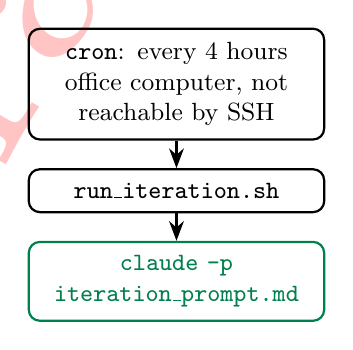
\begin{tikzpicture}[node distance=0.35cm]
    \node[box, text width=3.4cm] (c) {\texttt{cron}: every 4 hours\\ office computer, not reachable by SSH};
    \node[box, text width=3.4cm, below=of c] (r) {\datei{run\_iteration.sh}};
    \node[box, draw=lauf, text=lauf, text width=3.4cm, below=of r] (l) {\texttt{claude -p}\\ \datei{iteration\_prompt.md}};
    \draw[pfeil] (c) -- (r);
    \draw[pfeil] (r) -- (l);
  \end{tikzpicture}
  \hfill
  \begin{minipage}[c]{0.6\textwidth}
    \begin{enumerate}
    \setlength\itemsep{2pt}
    \item \textbf{Lock} (\texttt{flock}): runs never overlap.
    \item \textbf{Set \texttt{PATH}}: otherwise \texttt{cron} cannot find \texttt{claude}.
    \item Write \datei{STATUS.md}, commit and push: the heartbeat.
    \item \texttt{claude -p} with a \textbf{hard time limit} (90, later 180 minutes)
      and a \textbf{narrow tool list}: \texttt{python3}, \texttt{git},
      \texttt{pdftotext}, \texttt{ls}, \dots
    \item Commit and push \textbf{even on failure}.
    \item Keep the logs of the last 60 runs.
    \end{enumerate}
    \medskip
    Anything not allowed is refused, not asked about, so a run never waits for me.
    I switched off system suspend on the machine.
  \end{minipage}
\end{frame}

% ------------------------------------------------------------------
\begin{frame}{Misstep 1: the run would never have started}
  The trial run on the morning of 3 Aug found \textbf{four errors}, each of which would
  have killed the unattended run at once:
  \begin{itemize}
  \item The repository was not at the path the script expected:
    \texttt{cd} fails, the script exits, no log.
  \item An \texttt{--add-dir} pointing to a missing directory: \texttt{claude} aborts
    immediately.
  \item The GPU simulation was somewhere other than stated.
  \item An unnecessary \texttt{venv} instruction.
  \end{itemize}
  \medskip
  \textbf{More important for the content:} \datei{Papers/ratchet/} held far more than
  \datei{PROBLEM.md} knew about, including \datei{ldp.tex} with the Hamiltonian already
  derived. Without an entry, the run would have rebuilt it. Since then every file is listed
  in the problem statement, with a checked \enquote{file $\mapsto$ paper} assignment.
\end{frame}

% ------------------------------------------------------------------
\begin{frame}{Misstep 2: a numerics machine}
  \small
  \begin{columns}[T]
    \begin{column}{0.48\textwidth}
      \textbf{How it was set up}
      \begin{itemize}
      \item \datei{PROBLEM.md}: the simulation as \enquote{verifier (binding)}
      \item prompt: \enquote{check numerically}
      \item three kinds of result, all ranked equally
      \end{itemize}
      \textbf{Iteration 1} produced four good measurements, no attempt at a proof, and
      proposed something numerical again.
    \end{column}
    \begin{column}{0.5\textwidth}
      \textbf{Supervisor's note}, 3 Aug, added to the log by hand, \emph{not} an
      iteration:
      \begin{itemize}
      \item \textbf{The goal is a theorem, not a table.}
      \item The simulation is a \textbf{sanity check}: it can refute, never
        confirm. Anything only supported numerically stays a CONJECTURE.
      \item $V_\ast$ is an infimum, so bounds need \textbf{no} LDP:
      \end{itemize}
      \footnotesize
      \textbf{B1}: every path $\varphi$ gives $V_\ast\le I(\varphi)$.\\
      \textbf{B2}: every subsolution $F$ gives $V_\ast\ge\inf\{F: x_0=0\}$.
    \end{column}
  \end{columns}
  \bigskip
  Iteration 2 then proved a negative result: the $(x_0,m_1)$ closure gives no lower
  bound.
\end{frame}

% ------------------------------------------------------------------
\begin{frame}{Iterations 1--39: bounds on $V_\ast$ (3--9 Aug)}
  \begin{itemize}
  \setlength\itemsep{3pt}
  \item Up to six runs a day, each ending with a theorem, a negative result or a
    justified dead end.
  \item Examples: iteration~5, \enquote{no moment closure of finite order gives a lower
    bound}; iteration~6, the entropy approach refuted; iteration~9, \textbf{the first
    proved positive lower bound} for $\theta>1$.
  \item State after 39 iterations: $V_\ast$ bracketed to within $\pm20\,\%$ for
    $\theta\lesssim2$. This became \datei{paper/quasipotential.tex}.
  \end{itemize}
  \begin{block}{Misstep 3: the book nobody opened}
    \footnotesize
    Iteration~39 no longer improved a number at any $\theta$. A search of the log found
    \textbf{zero} hits for \enquote{Dawson}, \enquote{Kurtz},
    \enquote{comparison principle}, \enquote{tightness}. Dawson \& Feng had been available
    locally from the start. This followed from the setup: the problem statement
    deliberately bypassed the LDP. The runs work through what is written down, and do not
    ask whether it is still the right thing.
  \end{block}
\end{frame}

% ------------------------------------------------------------------
\begin{frame}{The change of course: tailored series (from 12 Aug)}
  \footnotesize
  \begin{tabular}{@{}llllp{0.37\textwidth}@{}}
    \toprule
    Series & Iterations & Dates & Goal & Result \\
    \midrule
    B1--B3 & 1--39 & 3--9 Aug & bounds on $V_\ast$ & bracketed, $\pm20\,\%$ \\
    B4 & 40--46 & 12--14 Aug & the LDP itself & path LDP on a fixed horizon (Thm.~46.4) \\
    B5 & 47--52 & 14--15 Aug & the actual click, $\varepsilon\to0$ & $P(\text{click before }T)=e^{-n(v_T+o(1))}$ \\
    B6 & 53--54 & 17 Aug & the time horizon & $\lim_T v_T=V_\ast$ (Thm.~53.4) \\
    B7 & 55--74 & 18--23 Aug & the time scale & first click time on the scale $e^{nV_\ast}$; click-rate band \\
    B8 & 61 & 18 Aug & moderate deviations & negative after one run, closed \\
    \bottomrule
  \end{tabular}

  \bigskip
  \begin{itemize}
  \item Each series has a section in \datei{PROBLEM.md} with a fixed scope; for B4,
    \textbf{one method per run}. Each iteration delivers a self-contained theorem,
    \enquote{not a quarter four times over}.
  \item \texttt{RATCHET\_STOP\_AFTER}: the series ends by itself, so no run continues
    without a tailored task.
  \item After each iteration an addendum \enquote{task from it.~$N$ on}. This sets the
    named goal of the next run.
  \end{itemize}
\end{frame}

% ------------------------------------------------------------------
\begin{frame}{Three parties, and where the steering happens}
  \centering
  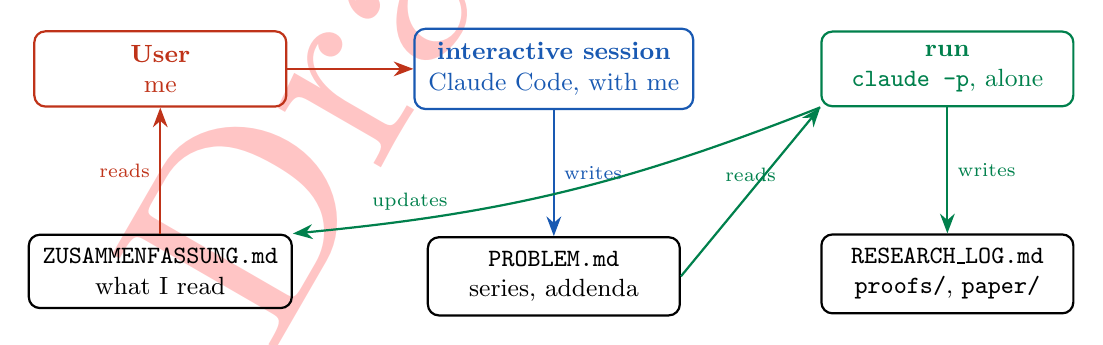
\begin{tikzpicture}[node distance=1.2cm and 1.6cm]
    \node[box, draw=nutzer, text=nutzer, minimum width=3.2cm] (N) {\textbf{User}\\me};
    \node[box, draw=sitzung, text=sitzung, minimum width=3.2cm, right=of N] (S)
      {\textbf{interactive session}\\Claude Code, with me};
    \node[box, draw=lauf, text=lauf, minimum width=3.2cm, right=of S] (L)
      {\textbf{run}\\\texttt{claude -p}, alone};

    \node[box, below=1.6cm of N, minimum width=3.2cm] (Z) {\datei{ZUSAMMENFASSUNG.md}\\what I read};
    \node[box, below=1.6cm of S, minimum width=3.2cm] (P) {\datei{PROBLEM.md}\\series, addenda};
    \node[box, below=1.6cm of L, minimum width=3.2cm] (R) {\datei{RESEARCH\_LOG.md}\\\datei{proofs/}, \datei{paper/}};

    \draw[pfeil, nutzer] (N) -- (S);
    \draw[pfeil, sitzung] (S) -- node[right, font=\scriptsize]{writes} (P);
    \draw[pfeil, lauf] (P.east) -- node[above, font=\scriptsize]{reads} (L.south west);
    \draw[pfeil, lauf] (L) -- node[right, font=\scriptsize]{writes} (R);
    \draw[pfeil, lauf] (L.south west) to[bend left=8] node[pos=0.8, above, font=\scriptsize]{updates} (Z.north east);
    \draw[pfeil, nutzer] (Z) -- node[left, font=\scriptsize]{reads} (N);
  \end{tikzpicture}

  \medskip
  \small
  \begin{itemize}
  \item \textbf{Supervisor's notes} in the log, explicitly \enquote{not an iteration}:
    they override the proposed next step.
  \item Since 12 Aug every iteration updates \datei{ZUSAMMENFASSUNG.md} (the summary),
    about ten pages: the only thing a human reads. \datei{FORTSCHRITT.pdf} ended up at
    840 pages.
  \end{itemize}
\end{frame}

% ------------------------------------------------------------------
\begin{frame}{Missteps in operation}
  \scriptsize
  \begin{tabular}{@{}lp{0.44\textwidth}p{0.36\textwidth}@{}}
    \toprule
    Date & Failure & afterwards \\
    \midrule
    12 Aug & The stop limit also counted failed runs: a run dying at the usage limit
              used up a slot of the series & only \texttt{rc=0} counts \\
    12 Aug & Page images from a 414-page book eat the quota &
              \texttt{pdftotext} by default \\
    15--20 Aug & Of 27 slots, 21 died at the limit, 19 of them at \enquote{Fable~5 limit},
              without computing for a single second. \texttt{--fallback-model} does not
              help with that & runner switched to Opus~5 \\
    20 Aug & \enquote{session limit} not recognised and reported as a repository error &
              pattern added \\
    20 Aug & A run stopped by the time limit left no trace: \enquote{nothing gets lost}
              was wrong & first commit within 20 minutes, then one per step \\
    21 Aug & A one-off crontab entry for 21 Aug would have fired again in 2027 &
              removed by hand \\
    23 Aug & Iteration~73 did not write the addendum with the next task & added by
              hand \\
    \bottomrule
  \end{tabular}

  \medskip
  87 runs: 63 regular, 24 with an error, almost all at the quota.
  74 iterations in terms of content, some of them started by hand.
\end{frame}

% ------------------------------------------------------------------
\begin{frame}{Missteps in the mathematics}
  \small
  \textbf{Refuted and documented: this is the normal case}
  \begin{itemize}
  \item The entropy approach to B2 (it.~6): it breaks at the threshold $\theta_c=2.4088$.
  \item (R59-a) refuted and repaired (20 Aug): the product $x_0m_1$ instead of the pair
    $(x_0,m_1)$.
  \item The clause (K1) refuted (it.~72), followed by two new routes.
  \item B8 (moderate deviations): negative after one run.
    $c_{MD}\sim1/(2\log\theta)\to0$ instead of a value in $(0,1)$. The series had been
    planned for six runs.
  \end{itemize}
  \textbf{Found only when proofreading by hand} (22 Aug, five findings, no statement falls)
  \begin{itemize}
  \item The introduction claimed a full limit. It is proved only under the hypothesis
    (RET).
  \item A comparison function solved the wrong Riccati equation: the difference is exactly
    $\theta/2$.
  \item A constant cited with $\delta/4$ instead of $\delta/8$. One bound was
    \emph{smaller} than the one proved.
  \end{itemize}
  The runs check their own proofs, but check the \textbf{chains of citations} between
  iterations poorly.
\end{frame}

% ------------------------------------------------------------------
\begin{frame}{What came out (as of 25 Aug)}
  \small
  \begin{tabular}{@{}lrp{0.6\textwidth}@{}}
    \toprule
    Manuscript & Pages & Content \\
    \midrule
    \datei{ldp.tex} & 75 & path LDP on a fixed horizon; the actual click; $v_T\downarrow V_\ast$;
                         first click time on the scale $e^{nV_\ast}$ \\
    \datei{clickrate.tex} & 16 & $\liminf_n\frac1n\log\liminf_t K^\ast(t)/t\ge-V_\ast$,
                         unconditionally and a.s.; the upper half under (RET) \\
    \datei{quasipotential.tex} & 22 & B1--B3: bounds on $V_\ast$ without an LDP \\
    \datei{rate.tex} & 6 & the one-dimensional reduction (it.~52) \\
    \bottomrule
  \end{tabular}

  \bigskip
  \begin{itemize}
  \item Planned for one week, it ran for three (3--23 Aug).
  \item Open: (RET), the existence of $\mathfrak r$, the path LDP in $D_\infty$ via
    Dawson--Gärtner.
  \item \datei{paper/LEAN\_TODO.md} (18 Aug): \datei{ldp.tex} cannot be formalised today;
    parts of \datei{quasipotential.tex} can.
  \end{itemize}
\end{frame}

% ------------------------------------------------------------------
\begin{frame}{What I learned}
  \begin{itemize}
  \setlength\itemsep{6pt}
  \item \textbf{The problem statement is the lever.} Both big missteps, the numerics
    machine and the unopened book, were written into \datei{PROBLEM.md}. The runs did
    exactly what it said.
  \item \textbf{Direction stays with the user.} A run does not notice that a route is
    exhausted. It only refines it.
  \item \textbf{Tailoring beats freedom.} Since the series, each run has a named goal and a
    stop limit, and within two weeks the LDP became a manuscript.
  \item \textbf{A verifier that can only refute is not enough.} The proofs were written in
    prose. What actually carries them only showed up in proofreading.
  \item \textbf{Operations cost more than expected.} Paths, quotas, stop counters and
    leftover crontab entries: each of these failures happened once and has been a comment
    in the script ever since.
  \end{itemize}
\end{frame}

\end{document}
